\subsection{Introduction}
\begin{description}
    \item[Random Numbers] Random numbers are sequence of statistically
        independent and unbiased numbers.
    \item[Random Bits] Random bits are a sequence of statistically independent
        and unbiased binary digits.
    \item[Uniform distribution] All the numbers in a given range must occur
        equally often.
    \item[Independence] Given the knowledge of the all previous numbers
        generated, you can not predict the next number.
\end{description}

\subsubsection{Entropy}
The entropy is used to describe a measure of randomness, a description
of how hard a value is to guess.

\begin{itemize}
    \item Let us assume that $X$ is a discrete random variable on the sample
        space $ \Omega_n = \{\omega_1,\omega_2,\ldots,\omega_n\} $ with the
        probability distribution $P=\{ p_i,1 \leq i \leq n \}$. The entropy $H(X)$
        of X is defined by:
        $$ H(X)= - \sum_{i=1}^{n} p_i \log_{2}p_i $$
\end{itemize}

\subsubsection{Kolmogorov}
The idea of Kolmogorov is to measure the randomness with the
complexity of the minimal program (Turing machine) that
generates a sequence

\subsubsection{Common Uses} 
\begin{itemize} 
    \item Randomness is needed for key generation, nonces, salt,\ldots
    \item[Note] A random number can do the job of an arbitrary number. The
        reverse is not true
\end{itemize}

\subsection{Generating Randomness}
\begin{description}
    \item[Random bit Generator] A random bit generator is a device or algorithm
        which outputs a sequence of statistically independent and unbiased binary
        digits.

        \begin{itemize}
            \item[$\Rightarrow$] A random integer in the interval [0;n] can be obtained by
                generating a random bit sequence of length $ \lfloor
                \log_2{}{n} \rfloor + 1 $
                and converting it to an integer.
        \end{itemize}
\end{description}

\begin{center}
    \textit{Anyone who attempts to generate random numbers by
    deterministic (predictable, reproducible) means is, of course, living in a state of sin.}
\end{center}


\subsection{Hardware Random Number Generators}
The source of entropy come the software (time, process ID, user) or the hardware
(mechanical noises, electrical noises).

\subsubsection{Random Number Generators}
\begin{tabular}{m{13cm}m{3cm}}
    \begin{itemize}
        \item\textbf{Non-deterministic RNGs} (True RNGs): Each bit produced by a HRNG comes
            from the observation of an unpredictable physical process.
        \item\textbf{Deterministic RNGs} (PRNG): Each bit is produced by a deterministic
            algorithm properly initialized.
    \end{itemize}
    &
    \begin{tikzpicture}[node distance=0.5cm]
        \node[draw, rectangle] (A) {TRNG};
        \node[draw, rectangle, below =of A] (C) {PRNG};
        \node[below=of C] (D) {output};

        \path[->] (A) edge (C)
        (C) edge (D);
    \end{tikzpicture}
\end{tabular}

\subsection{PRNGs in Theory}
\begin{description}
    \item[Pseudo Random Bit Generator] A PRBG is a deterministic algorithm
        which given a truly random binary sequence of length $k$, outputs a binary
        sequence of length $l \gg k $ which \textbf{appears} to be random. 
        \begin{center}
            \begin{tikzpicture}[node distance=0.5cm]
                \node[draw, rectangle] (A) {Seed};
                \node[draw, rectangle, right =of A] (C) {PRNG};
                \node[right=of C] (D) {pseudo-random bit sequence};

                \path[->] (A) edge (C)
                (C) edge (D);
            \end{tikzpicture}
        \end{center}

        \begin{itemize}
            \item The output of PRBG is not random as the number of
                possible output sequences is at most a small
                fraction, namely $2^k$, of all possible binary
                sequences of length $l$
        \end{itemize}

    \item[PRNG-FSM] A PRNG is a FSM defined by: $$x_{t+1} = f(x_t)$$ 
        $f$ is the transition function and $x_0$ is the seed.
    \item[Period] The period T of the PRNG is the smallest integer such that:
        $x_{t+T} = x_t$
\end{description}

\subsubsection{Generator method}
\begin{itemize}
    \item \textbf{Middle-square Method}

        \begin{tabular}{m{11cm}m{6cm}}
            To generate a sequence of $n$-digit pseudo-random numbers:
            \begin{enumerate}
                \item A $n$-digit seed is created and squared
                \item Middle $n$ digits of the result are output 
                \item The output is know the seed of the process
            \end{enumerate}
            &
            Example with $n$= 6

            \begin{tikzpicture}[node distance=0.5cm]
            \node (firstseed){\begin{tabular}{c}847209\\seed\end{tabular}};
                \node (result)[below=of
                firstseed]{\begin{tabular}{c}717\textcolor{red}{763089}681\\
                seed$^2$\end{tabular}};
                \node (result2)[below=of result]{763089};

                \draw[->] (firstseed) -- (result);
                \draw[->] (result) -- (result2);
                \draw[->] (result2) -| (+1.5cm, +0cm) |- (firstseed);
            \end{tikzpicture}
        \end{tabular}

        \paragraph{Inconvenients}

        \begin{itemize}
            \item For a generator of n-digits numbers, the period cannot be longer than
                $10^n$.
            \item If the middle n digits are all zeroes, the generator then outputs
                zeroes forever.
            \item If the first half of the middle n digits are all zeroes, the
                subsequent values decrease to zero.
            \item There exists short periods.
        \end{itemize}

    \item \textbf{Linear Congruential Generator} A LCG produces a pseudorandom sequence
        of numbers $x_1,x_2,x_3,\ldots$ according to the linear recurrence:
        $$ x_n = a\times x_{n-1} + b \quad \mod{m}\quad with\ n \geq 1 $$

        The integers $a$ (multiplier), $b$ (increment), and $m$ (modulus) are parameters
        which characterize the generator while $x_0$ is the (secret) seed.

        \begin{itemize}
            \item $m$ defines the maximum possible cycle
                length
            \item $a$ defines the number of cycles 
        \end{itemize}

        \begin{tabular}{m{8cm}m{6cm}}
            $$x_{t+1} = \textcolor{red}{5} x_t \quad mod\quad 13$$
            &
            $$x_{t+1} = \textcolor{red}{6} x_t \quad mod\quad 13$$
            \\

            \begin{scriptsize}
                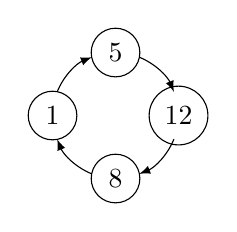
\begin{tikzpicture}
                    \def \n {4}
                    \def \radius {0.8cm}
                    \def \margin {22} % margin in angles, depends on the radius
                    \foreach \s/\r in {1/12, 2/5, 3/1, 4/8} {
                        \node[draw, circle] at ({360/\n * (\s - 1)}:\radius) {$\r$};
                        \draw[<-, >=latex] 
                        ({360/\n * (\s - 1)+\margin}:\radius) 
                        arc 
                        ({360/\n * (\s - 1)+\margin}:{360/\n * (\s)-\margin}:\radius);
                    }
                \end{tikzpicture}
                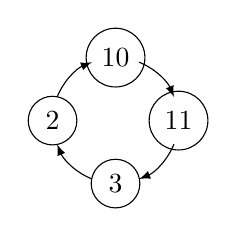
\begin{tikzpicture}
                    \def \n {4}
                    \def \radius {0.8cm}
                    \def \margin {22} % margin in angles, depends on the radius
                    \foreach \s/\r in {1/11, 2/10, 3/2, 4/3} {
                        \node[draw, circle] at ({360/\n * (\s - 1)}:\radius) {$\r$};
                        \draw[<-, >=latex] 
                        ({360/\n * (\s - 1)+\margin}:\radius) 
                        arc 
                        ({360/\n * (\s - 1)+\margin}:{360/\n * (\s)-\margin}:\radius);
                    }
                \end{tikzpicture}
                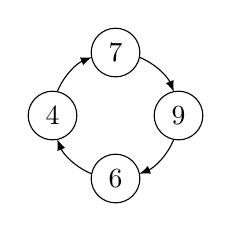
\begin{tikzpicture}
                    \def \n {4}
                    \def \radius {0.8cm}
                    \def \margin {22} % margin in angles, depends on the radius
                    \foreach \s/\r in {1/9, 2/7, 3/4, 4/6} {
                        \node[draw, circle] at ({360/\n * (\s - 1)}:\radius) {$\r$};
                        \draw[<-, >=latex] 
                        ({360/\n * (\s - 1)+\margin}:\radius) 
                        arc 
                        ({360/\n * (\s - 1)+\margin}:{360/\n * (\s)-\margin}:\radius);
                    }
                \end{tikzpicture}


            \end{scriptsize}
            &

            \begin{scriptsize}
                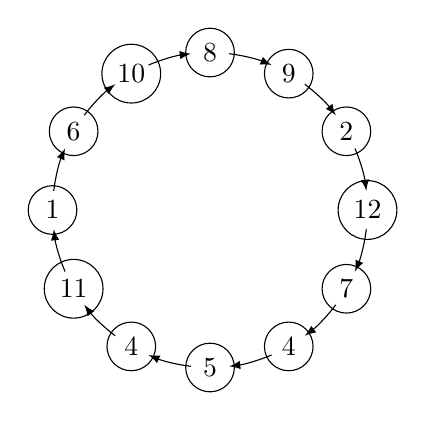
\begin{tikzpicture}
                    \def \n {12}
                    \def \radius {2.0cm}
                    \def \margin {7} % margin in angles, depends on the radius
                    \foreach \s/\r in {1/12, 2/2, 3/9, 4/8, 5/10,
                    6/6, 7/1, 8/11, 9/4, 10/5, 11/4, 12/7} {
                        \node[draw, circle] at ({360/\n * (\s - 1)}:\radius) {$\r$};
                        \draw[<-, >=latex] 
                        ({360/\n * (\s - 1)+\margin}:\radius) 
                        arc 
                        ({360/\n * (\s - 1)+\margin}:{360/\n * (\s)-\margin}:\radius);
                    }
                \end{tikzpicture}
            \end{scriptsize}
        \end{tabular}

        \paragraph{Predictable}
        As LCGs is predictable, they are used for simulation purpose and probabilistic
        algorithms but it's insecure
        for cryptographic purpose!

        $\Rightarrow$ Given a partial output sequence, the remainder of
        the sequence can be reconstructed even if the parameters $a$, $b$,
        and $m$ are unknown.

    \item \textbf{Lehmer RNG}: variant of LCG where $m$ is a prime
        number or a power of a prime number and $b=0$
        $$ x_n = a\times x_{n-1}  \quad \mod{m}\quad with\ n \geq 1 \
        and\ m\ prime\ or\ power\ of\ a\ prime $$

        \begin{itemize}
            \item if $a=0 \Rightarrow \forall_t f(x_t)=0$, we have a fixed point
            \item if $a=1 \Rightarrow \forall_t f(x_t)=x_0$, we have a fixed point
                \item if $a=2$, whe have a od-even pattern
                    \end{itemize}

    \item \textbf{Blum-Blum-Shub Generator}
        \begin{itemize}
            \item Let $m=p\times q$ where 
                \begin{enumerate}
                        \item p and q are both primes congruent to 3 modulo
                4 ($p \equiv 3 mod 4$)
                        \item and $ \gcd{\big(\phi(p)}{\phi(q)\big)} $
                            is small. ($\phi(p) = |\{ n < p \wedge n
                                \textrm{ prime with } p$ )
                            \end{enumerate}
                $$\begin{cases}
                        x_0 & = \textrm{seed}\\
                        x_{n+1} & = x^2_n\ \mod{m}
                        \end{cases}$$
            \item We output the parity bit of $x_n$ $(n>0)$.
        \end{itemize}

        \paragraph{Comment}
        It is always safe to use only the lowest order bit. 
        \begin{itemize}
            \item If you use no more than the $log_2 (log_2 (x_n ))$ low order bits, then predicting
                any additional bits from a sequence generated in this manner is
                provable as hard as factoring $m$. 
            \item As long as the initial $x_0$ is secret,
                you can even make $m$ public if you want.
        \end{itemize}

    \item \textbf{ANSI X9.17}: mostly used PRNG 

        \begin{itemize}
            \item Input: a random (and secret) 64-bit seed $x_0$ and a integer $m$
            \item Output: $m$ pseudo-random 64-bit string $x_1,x_2,\ldots,x_m$
                $$x_{t+1} = E_k\bigg(\underbrace{E_k(time())}_{T_t}
                \quad \oplus \quad \underbrace{E_k(x_t \oplus
                T_t)}_{o_t}\bigg)$$
            \item[Note] that $E_k$ is a DES (E-D-E two-key
                triple-encryption) with key $k$
        \end{itemize}

        ANSI X9.17 is fast but there is no security proof (under
        reasonable assumption) that it's a secure PRNG

    \item \textbf{LFSR}
        \begin{center}
            \begin{tikzpicture}
                \node [shape = rectangle](b3) {$b_3$};
                \node [shape = rectangle, right=of b3] (b2) {$b_2$};
                \node [shape = rectangle, right=of b2] (b1) {$b_1$};
                \node [shape = rectangle, above=0.5cm of b1] (xor) {$\oplus$};
                \node [shape = rectangle, right=of b1] (b0) {$b_0$};
                \node [right=of b0] (c) {\begin{tabular}{c}Add to
                pseudo-\\random sequence\end{tabular}};


                \draw [->] (b3) -- (b2);
                \draw [->] (b2) -- (b1);
                \draw [->] (b1) -- (b0);
                \draw [->] (b1) -- (xor);

                \draw[->] (b0) |- (xor);
                \draw [->] (xor) -| (b3);
                \draw[->] (b0) -- (c);
            \end{tikzpicture}
        \end{center}

\end{itemize}


\subsection{PRNGs in practice}

\subsubsection{Apple Carbon Library}
$$x_{t+1} = 16807 \times x_t \mod 2^{31} -1 $$

\begin{itemize}
    \item Need to be careful with \textbf{overflow}. 
        When you multiply 2 n-bit numbers, the results is on 2n bits.
        \end{itemize}

\subsubsection{UNIX Rand}
$$x_{t+1} = (1103515245 \times x_t) + 12345 \mod 2^{31}$$
\paragraph{Note} This generator is heavily \textbf{biased}!

\begin{lstlisting}[frame=single,language=C]
while(i){
	//set seed to time(NULL), time() return time in ms
	srandom(time(NULL)); 
	//print random number
	printf(''\%d,random()'');
}
\end{lstlisting}
\begin{itemize}
    \item[$\Rightarrow$] If the processor is in GHz , time() will return the
        same value during a certain period of time.
\end{itemize}

%TODO /dev/random /dev/urandom ?

\subsection{Implementation}

A PRNG is roughly defined by 3 functions: \begin{tabular}{ll}
    \texttt{instantiate()} & : defines a unique instance of a PRNG.\\
    \texttt{generate()} & :  produces the random number from the seed.\\
    \texttt{test()} & : tests the randomness of everything.\\
\end{tabular}
